\documentclass[a4j, dvipdfmx]{jsarticle}

\usepackage[square,numbers]{natbib}
% \usepackage[backend=biber]{biblatex}
\usepackage{mathtools}
\usepackage{amsmath, amsthm , amssymb, amscd}
\usepackage{ascmac}
\usepackage{physics}
\usepackage{here}
\usepackage{url}
\usepackage{bm}
\usepackage{tcolorbox}
\usepackage{algorithm, algpseudocode}
\usepackage{color}
\usepackage{xcolor}

\title{
    PGMLLL: 新しい多項式時間で停止するLLL with deep-insertionsの提案
    \\
    PGMLLL: A Development of A New Polynomial-time Variant of LLL with Deep-insertions
}
\author{
    さとしん
    \\
    立教大学大学院
}
\markright{さとしん}
\pagestyle{myheadings}

\theoremstyle{definition}
\newtheorem{definition}{Definition}[section]
\newtheorem{proposition}[definition]{Proposition}
\newtheorem{lem}[definition]{Lemma}
\newtheorem{theorem}[definition]{Theorem}
\newtheorem{corollary}[definition]{Corollary}
\newtheorem{rem}[definition]{Remark}
\newtheorem{fact}[definition]{Fact}
\newtheorem{note}[definition]{Note}
\newtheorem{ex}[definition]{Example}

\newcommand{\round}[1]{\left\lfloor #1\right\rceil}
\newcommand{\bhline}{\noalign{\hrule height 1.0pt}}

\begin{document}
\maketitle

\section{準備}

\subsection{記号の準備}

本記事で使用する記号は以下の表に従う.

\begin{tabular}{l||l}
    記号 & 意味\\
    \bhline
    $\mathbb{Z}$ & 整数全体の集合\\
    \hline
    $\mathbb{Q}$ & 有理数全体の集合\\
    \hline
    $\mathbb{R}$ & 実数全体の集合\\
    \hline
    $\mathrm{M}_n(R)$ & 環$R$上の$n\times n$行列全体の集合\\
    \hline
    $\boldsymbol{O}_{n, m}$ & $n\times m$の零行列\\
    \hline
    $\boldsymbol{E}_n$ & $n$次単位行列\\
    \hline
    $q^{(\text{num})}$, $q^{(\text{den})}$ & $q\in\mathbb{Q}$の分子,及び分母(必ずしも\textbf{既約分数とは限らない})\\
    \hline
    $\round{\bullet}$ & 実数の四捨五入
\end{tabular}

\section{格子}

\begin{definition}[格子]
一次独立な$n$本のベクトル$\boldsymbol{b}_1,\ldots,\boldsymbol{b}_n\in\mathbb{R}^n$(これを\textbf{基底ベクトル}と呼ぶ)の整数係数の一次結合全体の集合
\[
L=\mathcal{L}(\boldsymbol{b}_1,\ldots,\boldsymbol{b}_n):=\left\lbrace \left.\sum_{i=1}^na_i\boldsymbol{b}_i~\right|~a_1,\ldots.a_n\in\mathbb{Z}\right\rbrace
\]
を(完全階数な)\textbf{格子}と呼び,基底ベクトルの組$\{\boldsymbol{b}_1,\ldots,\boldsymbol{b}_n\}$を\textbf{基底}と呼ぶ.
また,基底ベクトルが全て整数ベクトルであるとき,$L$を\textbf{整数格子}と呼び,本記事では整数格子のみ扱う.
\end{definition}

\subsection{Gram-Schmidtの直交化法}

\begin{definition}[Gram-Schmidtの直交化]
$\{\boldsymbol{b}_1,\ldots,\boldsymbol{b}_n\}$を$n$次元格子$L$の基底とする.このとき
\[
\left\{\begin{aligned}\boldsymbol{b}_1^\star &:= \boldsymbol{b}_1, \\\boldsymbol{b}_i^\star &:= \boldsymbol{b}_i - \sum_{j=1}^{i-1} \mu_{i, j} \boldsymbol{b}_j^\star,~\mu_{i, j}:=\frac{\langle \boldsymbol{b}_i, \boldsymbol{b}_j^\star\rangle}{\| \boldsymbol{b}_j^\star \|^2}~(1 \leq j < i \leq n).\end{aligned}\right.
\]
で定義される$\boldsymbol{b}_1^\star,\ldots,\boldsymbol{b}_n^\star$を\textbf{Gram-Schmidtの直交化ベクトル},$\boldsymbol{U}\coloneqq (\mu_{i, j})_{i, j}$を\textbf{Gram-Schmidtの直交化係数行列}と呼ぶ.
\end{definition}

B1やB2の線形代数学で習うようなGram-Schmidtの直交化法そのものです.

\subsection{体積}

\begin{definition}[体積]
$L$を$n$次元格子として,$\{\boldsymbol{b}_1,\ldots,\boldsymbol{b}_n\}$を$L$の基底とする.更に,
\[
\boldsymbol{B}\coloneqq \mqty[\boldsymbol{b}_1\\\vdots\\\boldsymbol{b}_n]\in \mathrm{M}_n(\mathbb{Z})
\]
とする.このとき,
$$
\mathrm{vol}(L)\coloneqq \sqrt{\det(\boldsymbol{BB}^\top)}=\prod_{i=1}^n \norm{\boldsymbol{b}_i^\star}
$$
を$n$次元格子$L$の\textbf{体積}または\textbf{行列式}と呼ぶ.
\end{definition}

\subsection{LLL}

\begin{definition}[LLL簡約基底(Lenstra, Lenstra and Lovász, 1982)]
$\lbrace\boldsymbol{b}_1,\ldots,\boldsymbol{b}_n\rbrace$を$n$次元格子$L$の基底とします.このとき,$\lbrace\boldsymbol{b}_1,\ldots,\boldsymbol{b}_n\rbrace$が簡約パラメタ$\frac{1}{4}<\delta<1$に対して\textbf{LLL簡約されている}とは
$$
\begin{array}{lll}
(\textbf{サイズ簡約条件})&1\le{}^\forall j<{}^\forall i\le n,&\lvert\mu_{i, j}\rvert\le \frac{1}{2}\\
(\textbf{Lovász条件})&2\le{}^\forall k<n, &\delta\lVert \boldsymbol{b}_{k-1}^\star\rVert\le \lVert \pi_{k-1}(\boldsymbol{b}_k)\rVert^2\end{array}$$を満たすときを言います.
\end{definition}

Lovász条件の不等式は$$\lVert\boldsymbol{b}_k^\star\rVert\ge (\delta-\mu_{k, k-1}^2)\lVert \boldsymbol{b}_{k-1}^\star\rVert^2$$と同値であるので,この不等式の方をLovász条件と呼ぶこともあります.
LLL簡約基底を求めるアルゴリズムは,多項式時間で停止することが知られています.

\subsection{DeepLLL(LLL with deep-insertion)}

DeepLLL簡約はLLL簡約の自然な一般化であり,以下の様に定義されます.

\begin{definition}[DeepLLL簡約基底(Schnorr and Euchner, 1994)]
$\lbrace\boldsymbol{b}_1,\ldots,\boldsymbol{b}_n\rbrace$を$n$次元格子$L$の基底とします.このとき,$\lbrace\boldsymbol{b}_1,\ldots,\boldsymbol{b}_n\rbrace$が簡約パラメタ$\frac{1}{4}<\delta<1$に対して\textbf{DeepLLL簡約されている}とは
$$
\begin{array}{lll}
(\textbf{サイズ簡約条件})&1\le{}^\forall j<{}^\forall i\le n,&\lvert\mu_{i, j}\rvert\le \frac{1}{2}\\
(\textbf{deep-exchange条件})&1\le{}^\forall i<{}^\forall k\le n,&\delta\lVert \boldsymbol{b}_{i}^\star\rVert\le \lVert \pi_{i}(\boldsymbol{b}_k)\rVert^2
\end{array}
$$
を満たすときを言います.但し,写像
$$
\begin{array}{llclc}
\pi_\ell : &\mathbb{R}^n &\longrightarrow &\langle \boldsymbol{b}_1, \dots, \boldsymbol{b}_{\ell-1} \rangle_\mathbb{R}^\perp&=\langle \boldsymbol{b}_\ell^\star, \dots, \boldsymbol{b}_n^\star \rangle_\mathbb{R}\\
&\boldsymbol{x} &\longmapsto &\displaystyle\sum_{i = \ell}^n \frac{\langle \boldsymbol{x}, \boldsymbol{b}_i^\star \rangle}{ \| \boldsymbol{b}_i^\star \|^2 } \boldsymbol{b}_i^\star
\end{array}
$$
は$\mathbb{R}$ベクトル空間$\langle \boldsymbol{b}_1, \dots, \boldsymbol{b}_{\ell-1} \rangle_\mathbb{R}$の直交補空間への直交射影とします.
\end{definition}

\begin{definition}[deep-insertion]
$n$次元格子$L$の基底$\{\boldsymbol{b}_1,\ldots,\boldsymbol{b}_n\}$に対して,\textbf{deep-insertion}$\sigma_{i, k}$とは
$$
\sigma_{i, k}: \{\boldsymbol{b}_1,\ldots, \boldsymbol{b}_n\}\longmapsto \lbrace\ldots,\boldsymbol{b}_{i-1},\boldsymbol{b}_k,\boldsymbol{b}_i,\ldots,\boldsymbol{b}_{k-1},\boldsymbol{b}_{k+1},\ldots\rbrace
$$
で定義される写像である.
\end{definition}

しかし,DeepLLL基底を求めるアルゴリズムはLLLアルゴリズムとは異なり停止性は証明されておらず,潜在的にはsuper-exponentialな計算量をもつとされています(Gama and Nguyen, 2008).
また,deep-insertion後の基底のGram-Schmidtの直交化ベクトルについては次の定理が成立します.

\begin{theorem}[Yamaguchi and Yasuda, 2018]
$\{\boldsymbol{b}_1,\ldots,\boldsymbol{b}_n\}$を$n$次元格子$L$の基底とし,さらに別の$L$の基底を
$$
\{\boldsymbol{c}_1,\ldots,\boldsymbol{c}_n\}\coloneqq \sigma_{i, k}(\{\boldsymbol{b}_1,\ldots,\boldsymbol{b}_n\})
$$
とする.このとき,基底$\{\boldsymbol{c}_1,\ldots,\boldsymbol{c}_n\}$のGram-Schmidtの直交化情報$(C_j)_{1\le j\le n},~(\nu_{\ell, j})_{1\le \ell, j\le n}$は,$\{\boldsymbol{b}_1,\ldots,\boldsymbol{b}_n\}$のGram-Schmidtの直交化情報$(B_j)_j, (\mu_{\ell, j})$及び$D_\ell\coloneqq \norm{\pi_\ell(\boldsymbol{b}_k)}^2$を用いて次のように表すことができる.
$$
C_j=\left\{
\!\!\!\!\!\!\begin{array}{lll}
& D_i & \text{if}~j=i\\
& \displaystyle\frac{D_jB_{j-1}}{D_{j-1}} & \text{if}~i+1\le j\le k\\
& B_j & \text{else}
\end{array}
\right.
$$
$$
\nu_{\ell, j}=\left\{
\!\!\!\!\!\!\begin{array}{lll}
&\displaystyle\mu_{\ell-1, j-1}-\frac{\mu_{k, j-1}}{D_j}\sum_{h=j}^{\ell-1}\mu_{k, h}\mu_{\ell-1, h}B_h & \text{if}~i+1\le j\le k,~j+1\le \ell\le k\\
&\displaystyle \mu_{\ell, j-1}-\frac{\mu_{k, j-1}}{D_j}\sum_{h=j}^k \mu_{k, h}\mu_{\ell, h}B_h & \text{if}~i+1\le j\le k,~k+1\le \ell \le n\\
&\displaystyle \frac{1}{D_i}\sum_{h=i}^{\ell-1}\mu_{k, h}\mu_{\ell-1, h}B_h & \text{if}~j=i,~i+1\le \ell \le k\\
& \displaystyle \frac{1}{D_i}\sum_{h=i}^{k}\mu_{k, h}\mu_{\ell, h}B_h & \text{if}~j=i,~k+1\le \ell\le n\\
& \mu_{k, j} & \text{if}~\ell=i,~1\le j\le i-1\\
& \mu_{\ell-1, j} & \text{if}~i+1\le \ell\le k,~1\le j\le i-1\\
& \mu_{\ell, j} & \text{else}
\end{array}
\right.
$$
\end{theorem} 

\section{既存の多項式時間で停止するLLL with deep-insertions}

\subsection{PotLLL}

PotLLLはFontein, Schneider and Wagner, 2014で初めて提案されたLLL with deep-insertionsの変種で,格子基底のpotentialと呼ばれる量(定義 6)がLovász条件を満たさない2つの隣接する基底ベクトル$(\boldsymbol{b}_{k-1},\boldsymbol{b}_k)$を交換した際に単調減少することに着目し,基底のpotentialが単調に減少するdeep-insertionのみを施すことにより多項式時間で停止する様に完了したものです.

\begin{definition}[potential]
$\{\boldsymbol{b}_1,\ldots,\boldsymbol{b}_n\}$を$n$次元格子$L$の基底とし,$L_i$を基底$\{\boldsymbol{b}_1,\ldots,\boldsymbol{b}_i\}$で張られる$i$次元格子とする.このとき,
$$
\mathrm{Pot}(\boldsymbol{b}_1,\ldots,\boldsymbol{b}_n)\coloneqq \prod_{i=1}^n \mathrm{vol}(L_i)^2=\prod_{i=1}^n \norm{\boldsymbol{b}_i^\star}^{2(n-i+1)}
$$
を基底$\{\boldsymbol{b}_1,\ldots,\boldsymbol{b}_n\}$の\textbf{potential}と呼ぶ.
\end{definition}

また,PotLLL簡約基底とは以下のような基底を言います.

\begin{definition}[PotLLL簡約基底 (Fontein, Schneider and Wagner, 2014)]
$\{\boldsymbol{b}_1,\ldots,\boldsymbol{b}_n\}$を$n$次元格子$L$の基底とする.このとき,$\{\boldsymbol{b}_1,\ldots,\boldsymbol{b}_n\}$が簡約パラメタ\textbf{$\frac{1}{4}<\delta<1$についてPotLLL簡約されている},もしくは\textbf{$\delta$-PotLLL簡約されている}とは
$$
\begin{array}{lll}
(\textbf{サイズ簡約条件})&\le{}^\forall j<{}^\forall i\le n,&\lvert\mu_{i, j}\rvert\le \frac{1}{2}\\
&1\le{}^\forall i<{}^\forall k\le n,&\delta\cdot \mathrm{Pot}(\lbrace\boldsymbol{b}_1,\ldots,\boldsymbol{b}_n\rbrace)\le\mathrm{Pot}(\sigma_{i, k}(\lbrace\boldsymbol{b}_1,\ldots,\boldsymbol{b}_n\rbrace))\end{array}
$$
の$2$条件を満たすことを言う.
\end{definition}

\subsection{S$\!{}^2$LLL}

S$\!{}^2$LLLはYasuda and Yamaguchi, 2019によって提案された多項式時間で停止するLLL with deep-insertionの変種で,PotLLLはpotentialを減少させていましたが,S$\!{}^2$LLLは格子基底の\textbf{Gram-Schmditの直交化ベクトルの二乗和}と呼ばれる量がLovász条件を満たさない2つの隣接する基底ベクトル$(\boldsymbol{b}_{k-1},\boldsymbol{b}_k)$を交換した際に単調減少することに着目し,基底のGram-Schmditの直交化ベクトルの二乗和が単調に減少するdeep-insertionのみを施すことにより多項式時間で停止する様に改良したものです.

\begin{definition}[Gram-Schmditの直交化ベクトルの二乗和]
$\{\boldsymbol{b}_1,\ldots,\boldsymbol{b}_n\}$を$n$次元格子$L$の基底とし,$L_i$を基底$\{\boldsymbol{b}_1,\ldots,\boldsymbol{b}_i\}$で張られる$i$次元格子とする.このとき,
$$
\mathrm{SS}(\boldsymbol{b}_1,\ldots,\boldsymbol{b}_n)\coloneqq \sum_{i=1}^n\lVert \boldsymbol{b}_i^\star\rVert^2
$$
を基底$\{\boldsymbol{b}_1,\ldots,\boldsymbol{b}_n\}$の\textbf{Gram-Schmditの直交化ベクトルの二乗和}(\textbf{squared-sum of Gram-Schmdit lengths})と呼ぶ.
\end{definition}

\begin{definition}[S${\!}^2$LLL簡約基底 (Yasuda and Yamaguchi, 2019)]
$\{\boldsymbol{b}_1,\ldots,\boldsymbol{b}_n\}$を$n$次元格子$L$の基底とする.このとき,$\{\boldsymbol{b}_1,\ldots,\boldsymbol{b}_n\}$が簡約パラメタ\textbf{$0< \eta \le 1$についてS${\!}^2$LLL簡約されている},もしくは\textbf{$\eta$-S${\!}^2$LLL簡約されている}とは
$$
\begin{array}{lll}
(\textbf{サイズ簡約条件})&\le{}^\forall j<{}^\forall i\le n,&\lvert\mu_{i, j}\rvert\le \frac{1}{2}\\
&1\le{}^\forall i<{}^\forall k\le n,&\eta\cdot \mathrm{SS}(\lbrace\boldsymbol{b}_1,\ldots,\boldsymbol{b}_n\rbrace)\le\mathrm{SS}(\sigma_{i, k}(\lbrace\boldsymbol{b}_1,\ldots,\boldsymbol{b}_n\rbrace))\end{array}
$$
の$2$条件を満たすことを言う.
\end{definition}

\section{新しく提案する簡約PGMLLL}

\subsection{Gram-Schmidt幾何平均の積}

今回新しくLLL with deep-insertionの変種を提案するに当たって,新しい格子基底に対して定まる量を定義しました.具体的には,以下で定義されるものです.

\begin{definition}[Gram-Schmidt幾何平均の積]
$\{\boldsymbol{b}_1,\ldots,\boldsymbol{b}_n\}$を$n$次元格子$L$の基底とする.このとき,
$$
\mathrm{GM}_k(\{\boldsymbol{b}_1,\ldots,\boldsymbol{b}_n\})\coloneqq \left(\prod_{i=1}^{k} \norm{\boldsymbol{b}_i^\star}^2\right)^{\frac{1}{k}}\quad (1\le k\le n)
$$
を格子基底$\{\boldsymbol{b}_1,\ldots,\boldsymbol{b}_n\}$の\textbf{Gram-Schmidt幾何平均}(\textbf{Gram-Schmidt geometric mean})と呼ぶことにし,その積
$$
\begin{aligned}
\mathrm{PGM}(\{\boldsymbol{b}_1,\ldots,\boldsymbol{b}_n\})&\coloneqq \prod_{k=1}^n \mathrm{GM}_k(\{\boldsymbol{b}_1,\ldots,\boldsymbol{b}_n\})\\
&=\prod_{k=1}^{n}\left(\prod_{i=1}^{k} \norm{\boldsymbol{b}_i^\star}^2\right)^{\frac{1}{k}}\\
&=\prod_{i=1}^n \norm{\boldsymbol{b}_i^\star}^{\sum_{k=i}^n \frac{2}{k}}
\end{aligned}
$$
を\textbf{Gram-Schmidt幾何平均の積}(\textbf{potential of Gram-Schmidt geometric mean})と呼ぶことにする.
\end{definition}

\subsection{Gram-Schmidt幾何平均の積の性質}

この,格子基底のGram-Schmidt幾何平均の積は,次の性質を持っています.

\begin{proposition}
$\{\boldsymbol{b}_1,\ldots,\boldsymbol{b}_n\}$を$n$次元格子$L$の基底とする.このとき,隣り合う基底ベクトル$(\boldsymbol{b}_{k-1}, \boldsymbol{b}_k)$が簡約パラメタ$\delta\in \left(\frac{1}{4}, 1\right)$に関するLovász条件を満たさないとき,新しい$L$の基底を
$$
\{\boldsymbol{c}_1,\ldots,\boldsymbol{c}_n\}\coloneqq \{\boldsymbol{b}_1,\ldots,\boldsymbol{b}_{k-2},\boldsymbol{b}_k,\boldsymbol{b}_{k-1},\boldsymbol{b}_{k+1},\ldots, \boldsymbol{b}_n\}
$$
と定めると
$$
\mathrm{PGM}(\boldsymbol{c}_1,\ldots,\boldsymbol{c}_n)<\delta^{\frac{1}{k-1}}\cdot\mathrm{PGM}(\boldsymbol{b}_1,\ldots,\boldsymbol{b}_n)
$$
が成立する.
\end{proposition}

\begin{proof}
簡単のため,$B_i\coloneqq \norm{\boldsymbol{b}_i^\star}^2, C_i\coloneqq \norm{\boldsymbol{c}_i^\star}^2$とします.このとき,$(\boldsymbol{b}_{k-1},\boldsymbol{b}_k)$がLovász条件を満たさない,即ち$B_k<(\delta-\mu_{k, k-1}^2)B_{k-1}$であることから
$$
C_{k-1}=B_k+\mu_{k, k-1}^2B_{k-1}<\delta B_{k-1}
$$
が成り立ちます.従って,
$$
\begin{aligned}
\mathrm{PGM}(\boldsymbol{c}_1,\ldots,\boldsymbol{c}_n)&=\prod_{j=1}^n \left(\prod_{i=1}^j C_i\right)^\frac{1}{j}\\
&=\prod_{j=1}^{k-2} \left(\prod_{i=1}^j B_i\right)^\frac{1}{j}\times \left(\prod_{i=1}^{k-1} C_i\right)^\frac{1}{k-1}\times \prod_{j=k}^n \left(\prod_{i=1}^j B_i\right)^\frac{1}{j}\\
&< \prod_{j=1}^{k-2} \left(\prod_{i=1}^j B_i\right)^\frac{1}{j}\times \left(\delta\prod_{i=1}^{k-1} B_i\right)^\frac{1}{k-1}\times \prod_{j=k}^n \left(\prod_{i=1}^j B_i\right)^\frac{1}{j}\\
&=\delta^{\frac{1}{k-1}}\prod_{j=1}^n \left(\prod_{i=1}^j B_i\right)^\frac{1}{j}\\
&=\delta^{\frac{1}{k-1}}\cdot\mathrm{PGM}(\boldsymbol{b}_1,\ldots,\boldsymbol{b}_n).
\end{aligned}
$$
となります.
\end{proof}

\begin{proposition}
$\{\boldsymbol{b}_1,\ldots,\boldsymbol{b}_n\}$を$n$次元格子$L$の基底とし,$B_i\coloneqq \norm{\boldsymbol{b}_i^\star}^2$をGram-Schmidtの直交化ベクトルの二乗ノルムとする.このとき,以下が成立する.
$$
1\le{}^\forall i<{}^\forall k\le n,~\frac{\mathrm{PGM}(\sigma_{i, k}(\boldsymbol{b}_1,\ldots,\boldsymbol{b}_n))}{\mathrm{PGM}(\boldsymbol{b}_1,\ldots,\boldsymbol{b}_n)}=\prod_{j=i}^k \left(\frac{D_j}{B_j}\right)^\frac{1}{j}
$$
ただし,$D_j\coloneqq \norm{\pi_j(\boldsymbol{b}_k)}^2$であり,写像
$$
\begin{array}{llclc}
\pi_j : &\mathbb{R}^n &\longrightarrow &\langle \boldsymbol{b}_1, \dots, \boldsymbol{b}_{j-1} \rangle_\mathbb{R}^\perp&=\langle \boldsymbol{b}_j^\star, \dots, \boldsymbol{b}_n^\star \rangle_\mathbb{R}\\
&\boldsymbol{x} &\longmapsto &\displaystyle\sum_{i = j}^n \frac{\langle \boldsymbol{x}, \boldsymbol{b}_i^\star \rangle}{ \| \boldsymbol{b}_i^\star \|^2 } \boldsymbol{b}_i^\star
\end{array}
$$
は$\mathbb{R}$ベクトル空間$\langle \boldsymbol{b}_1, \dots, \boldsymbol{b}_{j-1} \rangle_\mathbb{R}$の直交補空間への直交射影とする.
\end{proposition}

\begin{proof}
定理1から以下が従います.
\begin{align*}
&\frac{\mathrm{PGM}(\sigma_{i, k}(\boldsymbol{b}_1,\ldots,\boldsymbol{b}_n))}{\mathrm{PGM}(\boldsymbol{b}_1,\ldots,\boldsymbol{b}_n)}\\
=&\frac{\displaystyle \prod_{j=1}^{i-1}\left(\prod_{\ell=1}^j B_\ell\right)^\frac{1}{j}\times \left(D_i\prod_{\ell=1}^{i-1}B_\ell\right)^\frac{1}{i}\times \prod_{j=i+1}^k\left(D_j\prod_{\ell=1}^{j-1}B_\ell\right)^\frac{1}{j}\times \prod_{j=k+1}^n \left(D_k\prod_{\ell=1}^{k-1}B_\ell\cdot \prod_{\ell=k+1}^j B_\ell\right)^\frac{1}{j}}{\displaystyle \prod_{j=1}^n\left( \prod_{\ell=1}^{j}B_\ell\right)^\frac{1}{j}}\\
=&\frac{D_i^\frac{1}{i}}{B_i^\frac{1}{i}}\times \prod_{j=i+1}^k \frac{D_j^\frac{1}{j}}{B_j^\frac{1}{j}}\times \prod_{j=k+1}^n\frac{D_k^\frac{1}{j}}{B_k^\frac{1}{j}}\\
=&\prod_{j=i}^k \left(\frac{D_j}{B_j}\right)^\frac{1}{j}\times \left(\frac{D_k}{B_k}\right)^{\sum_{j=k+1}^n\frac{1}{j}}\\
=&\prod_{j=i}^k \left(\frac{D_j}{B_j}\right)^\frac{1}{j}.\quad \square
\end{align*}
\end{proof}

\begin{corollary}
    $$
    P_{i, k}\coloneqq \frac{\mathrm{PGM}(\sigma_{i, k}(\boldsymbol{b}_1,\ldots,\boldsymbol{b}_n))}{\mathrm{PGM}(\boldsymbol{b}_1,\ldots,\boldsymbol{b}_n)}
    $$
    とする.このとき,
    $$
    P_{i, k}=\left(\frac{\norm{\boldsymbol{b}_k}^2-\sum_{j=1}^{i-1}\mu_{k, j}^2B_j}{B_i}\right)^\frac{1}{i}P_{i+1, k}
    $$
    が成立する.
\end{corollary}

\begin{proof}
    $$
    \begin{aligned}
    P_{i, k}&=\prod_{j=i}^k \left(\frac{D_j}{B_j}\right)^\frac{1}{j}\times \left(\frac{D_k}{B_k}\right)^{\sum_{j=k+1}^n\frac{1}{j}}\\
    &=\left(\frac{D_i}{B_i}\right)^\frac{1}{i}\prod_{j=i+1}^k \left(\frac{D_j}{B_j}\right)^\frac{1}{j}\times \left(\frac{D_k}{B_k}\right)^{\sum_{j=k+1}^n\frac{1}{j}}\\
    &=\left(\frac{D_i}{B_i}\right)^\frac{1}{i}P_{i+1, k}.
    \end{aligned}
    $$
    ここで,
    $$
    D_i=\norm{\pi_i(\boldsymbol{b}_k)}^2=\norm{\boldsymbol{b}_k}^2-\sum_{j=1}^{i-1}\mu_{k, j}^2B_j
    $$
    を代入して
    $$
    P_{i, k}=\left(\frac{\norm{\boldsymbol{b}_k}^2-\sum_{j=1}^{i-1}\mu_{k, j}^2B_j}{B_i}\right)^\frac{1}{i}P_{i+1, k}
    $$
    を得る.
\end{proof}

\subsection{PGMLLL}

このGram-Schmidt幾何平均の積とその性質(主に命題2)を利用してPGMLLL簡約基底を次のように定義します.

\begin{definition}
    $\lbrace\boldsymbol{b}_1,\ldots,\boldsymbol{b}_n\rbrace$を$n$次元格子$L$の基底とします.このとき,$\lbrace\boldsymbol{b}_1,\ldots,\boldsymbol{b}_n\rbrace$が簡約パラメタ$\frac{1}{4}<\delta<1$に対して\textbf{PGMLLL簡約されている}とは
    $$
    \begin{array}{lll}
    (\textbf{サイズ簡約条件})&1\le{}^\forall j<{}^\forall i\le n,&\lvert\mu_{i, j}\rvert\le \frac{1}{2}\\
    &1\le{}^\forall i<{}^\forall k\le n,&\delta^{\frac{1}{i}}\cdot \mathrm{PGM}(\lbrace\boldsymbol{b}_1,\ldots,\boldsymbol{b}_n\rbrace)\le\mathrm{PGM}(\sigma_{i, k}(\lbrace\boldsymbol{b}_1,\ldots,\boldsymbol{b}_n\rbrace))
    \end{array}
    $$
    を満たすときを言う
\end{definition}.

\subsection{PGMLLLアルゴリズム}

Algorithm 1に命題3,並びにその系を利用したPGMLLL簡約基底アルゴリズムを示す.
$$
\begin{array}{ll}
& \!\!\!\!\!\!\!\!\!\!\!\!\textbf{Algorithm~1}~\text{PGMLLL}(\delta): \text{簡約パラメタ}\delta\text{に関するPGMLLL基底簡約アルゴリズム}\\
& \!\!\!\!\!\!\!\!\!\!\!\!\textbf{Input}:~n\text{次元格子の基底}\{\boldsymbol{b}_1,\ldots,\boldsymbol{b}_n\}\\
& \!\!\!\!\!\!\!\!\!\!\!\!\textbf{Output}:~\delta\text{に関するPGMLLL簡約基底}\{\boldsymbol{b}_1,\ldots,\boldsymbol{b}_n\}\\
1 & (B_i)_{1\le i\le n}, (\mu_{i, j})_{1\le i, j\le n}\gets \texttt{gram\_schmidt}()\\
2 & k\gets 1\\
3 & \textbf{while}~k\le n~\textbf{do}\\
4 & \quad \textbf{for}~j=k-1~\text{downto}~1~\textbf{do}\\
5 & \quad\quad \texttt{size\_reduce}(k, j)\\
6 & \quad P\gets 1;~P_{\min}\gets 1\\
7 & \quad i\gets 1\\
8 & \quad \textbf{for}~j=k-1~\text{downto}~1~\textbf{do}\\
9 & \quad\quad P\gets P\cdot \left(\frac{B_k+\sum_{\ell=j}^{k-1}\mu_{k, \ell}^2B_\ell}{B_j}\right)^\frac{1}{j}\\
10 & \quad\quad \textbf{if}~P<P_{\min}~\textbf{then}\\
11 & \quad\quad\quad i\gets j\\
12 & \quad\quad\quad P_{\min}\gets P\\
13 & \quad \textbf{if}~\delta^{\frac{1}{i}} > P_{\min}~\textbf{then}\\
14 & \quad\quad \{\boldsymbol{b}_1,\ldots,\boldsymbol{b}_n\}\gets \sigma_{i, k}(\{\boldsymbol{b}_1,\ldots,\boldsymbol{b}_n\})\\
15 & \quad\quad \text{Gram-Schmidtの直交化情報の更新}\\
16 & \quad\quad k\gets i\\
17 & \quad \textbf{else}\\
18 & \quad\quad k\gets k+1
\end{array}
$$
但し,$\texttt{gram\_schmidt}()$は基底のGram-Schmidtの直交化ベクトルの二乗ノルムとGram-Schmidtの直交化係数行列(この$2$つをまとめて\textbf{Gram-Schmidtの直交化情報}と呼ぶことにする)を計算する関数,$\texttt{size\_reduce}(k, j)$はサイズ基底簡約アルゴリズム,$\texttt{updata\_gso\_deep\_insertion}(i, k)$はdeep-insertion$\sigma_{i, k}$を施した後のGram-Schmidtの直交化情報の更新アルゴリズムで,それぞれ以下のアルゴリズムの様になる.
$$
\begin{array}{ll}
& \!\!\!\!\!\!\!\!\!\!\!\!\textbf{Algorithm~2}~\text{gram\_schmidt}(): \text{Gram-Schmidtの直交化情報を求める}\\
& \!\!\!\!\!\!\!\!\!\!\!\!\textbf{Input}:~n\text{次元格子の基底}\{\boldsymbol{b}_1,\ldots,\boldsymbol{b}_n\}\\
& \!\!\!\!\!\!\!\!\!\!\!\!\textbf{Output}:~\{\boldsymbol{b}_1,\ldots,\boldsymbol{b}_n\}\text{のGram-Schmidt情報}(B_i)_i,~(\mu_{i, j})_{i, j}\\
1 & B\gets \boldsymbol{0}_n\\
2 & \mu \gets \boldsymbol{E}_n\\
3 & \boldsymbol{b}_1^\star\gets \boldsymbol{0}_n;~\cdots;~\boldsymbol{b}_n^\star\gets \boldsymbol{0}_n\\
4 & \textbf{for}~i=1~\text{to}~n~\textbf{do}\\
5 & \quad \boldsymbol{b}_i^\star\gets \boldsymbol{b}_i\\
6 & \quad \textbf{for}~j=1~\text{to}~i-1~\textbf{do}\\
7 & \quad\quad \mu_{i, j}\gets \frac{\langle\boldsymbol{b}_i, \boldsymbol{b}_j^\star\rangle}{B_j}\\
8 & \quad\quad \boldsymbol{b}_i^\star\gets \boldsymbol{b}_i^\star-\mu_{i, j}\boldsymbol{b}_j^\star\\
9 & \quad B_i\gets \norm{\boldsymbol{b}_i^\star}^2\\
10 & \textbf{return}~B, \mu
\end{array}
$$

$$
\begin{array}{ll}
& \!\!\!\!\!\!\!\!\textbf{Algorithm~3}~\text{size\_reduce}(i, j): \text{部分的なサイズ基底簡約}\\
& \!\!\!\!\!\!\!\!\textbf{Input}:~n\text{次元格子の基底}\{\boldsymbol{b}_1,\ldots,\boldsymbol{b}_n\},~\text{そのGram-Schmidtの直交化係数行列}(\mu_{i, j})_{i, j}\\
& \!\!\!\!\!\!\!\!\textbf{Output}:~\text{簡約された基底}\{\boldsymbol{b}_1,\ldots,\boldsymbol{b}_n\}\text{と更新されたGram-Schmidtの直交化係数行列}(\mu_{i, j})_{i, j}\\
1 & \textbf{if}~\abs{\mu_{i, j}}>\frac{1}{2}~\textbf{then}\\
2 & \quad q\gets \round{\mu_{i, j}}\\
3 & \quad \boldsymbol{b}_i\gets \boldsymbol{b}_i-q\boldsymbol{b}_j\\
4 & \quad \textbf{for}~\ell=1~\text{to}~j~\textbf{do}\\
5 & \quad\quad \mu_{i, \ell}\gets \mu_{i, \ell}-q\mu_{j, \ell}
\end{array}
$$

\subsection{PGMLLLの計算量}

まず,PGMLLLにおける$3$行目から始まる$\textbf{while}$文の呼び出し回数について次がわかります.

\begin{proposition}
    Algorithm 1に基底$\{\boldsymbol{b}_1,\ldots,\boldsymbol{b}_n\}$を入力したとして,$X\coloneqq \max\{\norm{\boldsymbol{b}_1}^2, \ldots,\norm{\boldsymbol{b}_n}^2\}$とする.このとき,Algorithm 1でdeep-insertionが行われる回数は高々$\mathcal{O}(n^2\log X)$である.
\end{proposition}

\begin{proof}
    Algorithm 1の$14$行目のdeep-insertionの呼び出し回数を$N$とします.Algorithm 1より,呼び出される各deep-insertion$\sigma_{i, k}$により,格子基底のGram-Schmidtの幾何平均の積を$\delta^{\frac{1}{i}}$倍ずつ減少させていきます.$\frac{1}{4}<\delta<1$であるから
    $$
    \frac{1}{4}<\delta<\delta^\frac{1}{2}<\delta^\frac{1}{3}<\cdots <\delta^\frac{1}{n}<1
    $$
    が成立します.従って,格子基底のGram-Schmidtの幾何平均の積は各deep-insertion毎に少なくとも$\delta^\frac{1}{n}$ずつ減少します.
    他方で,Gram-Schmidtの幾何平均の積の定義から
    $$
    \begin{aligned}
    \mathrm{PGM}(\{\boldsymbol{b}_1,\ldots,\boldsymbol{b}_n\})&= \prod_{k=1}^n \mathrm{GM}_k(\{\boldsymbol{b}_1,\ldots,\boldsymbol{b}_n\})\\
    &=\prod_{k=1}^{n}\left(\prod_{i=1}^{k} \norm{\boldsymbol{b}_i^\star}^2\right)^{\frac{1}{k}}\\
    &=\prod_{k=1}^n \mathrm{vol}(L_i)^\frac{1}{k}\ge 1
    \end{aligned}
    $$
    であることがわかります.従って,
    $$
    \delta^{\frac{N}{n}}\mathrm{PGM}(\{\boldsymbol{b}_1,\ldots,\boldsymbol{b}_n\})\ge 1
    $$
    です.よって,
    $$
    \begin{aligned}
    &\delta^{\frac{N}{n}}\mathrm{PGM}(\{\boldsymbol{b}_1,\ldots,\boldsymbol{b}_n\})\ge 1\\
    \iff& \frac{N}{n}+\log_{\delta}[\mathrm{PGM}(\{\boldsymbol{b}_1,\ldots,\boldsymbol{b}_n\})]\le 0\\
    \iff& N\le -n\log_\delta\left[\mathrm{PGM}(\{\boldsymbol{b}_1,\ldots,\boldsymbol{b}_n\})\right]
    \end{aligned}
    $$
    となります.ここで,
    $$
    \begin{aligned}
    \mathrm{PGM}(\{\boldsymbol{b}_1,\ldots,\boldsymbol{b}_n\})&=\prod_{k=1}^{n}\left(\prod_{i=1}^{k} \norm{\boldsymbol{b}_i^\star}^2\right)^{\frac{1}{k}}\\
    &\le \prod_{k=1}^{n}\left(\prod_{i=1}^{k} \norm{\boldsymbol{b}_i}^2\right)^{\frac{1}{k}}\\
    &\le \prod_{k=1}^n \left(X^k\right)^\frac{1}{k}=X^n
    \end{aligned}
    $$
    ですので,前の式と合わせて
    $$
    \begin{aligned}
    N&\le -n\log_\delta\left[\mathrm{PGM}(\{\boldsymbol{b}_1,\ldots,\boldsymbol{b}_n\})\right]\\
    &=n\log_{\frac{1}{\delta}}\left[\mathrm{PGM}(\{\boldsymbol{b}_1,\ldots,\boldsymbol{b}_n\})\right]\\
    &\le n\log_\frac{1}{\delta} X^n
    \end{aligned}
    $$
    となります.従って,総回数$N$は高々$\mathcal{O}(n^2\log X)$です.
\end{proof}

\section{PGMLLLの実装 and 実験}

今回は$\texttt{SageMath}$ではなく,$\texttt{C++}$で$\texttt{NTL}$ライブラリを用いて実装しました.実際のコードは
%[$\texttt{https://github.com/satoshin-des/PGMLLL}$](https://github.com/satoshin-des/PGMLLL)
を見ていただくか,本記事の末尾をご覧ください.
\subsection{PGMの挙動}

まず,80次元におけるSVP Challengeのseed0の基底に関してPGMの挙動をプロットしました.それが以下の図たちです.

\begin{figure}[H]
    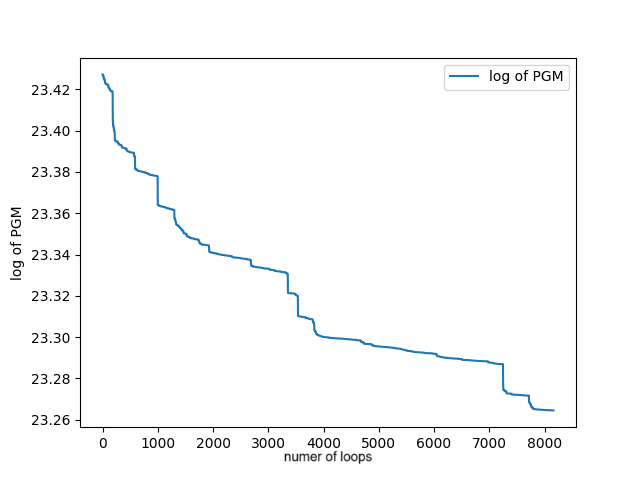
\includegraphics[width=100mm]{80.png}
    \caption{$80$次元における$\log \mathrm{PGM}$の挙動}
\end{figure}

\begin{figure}[H]
    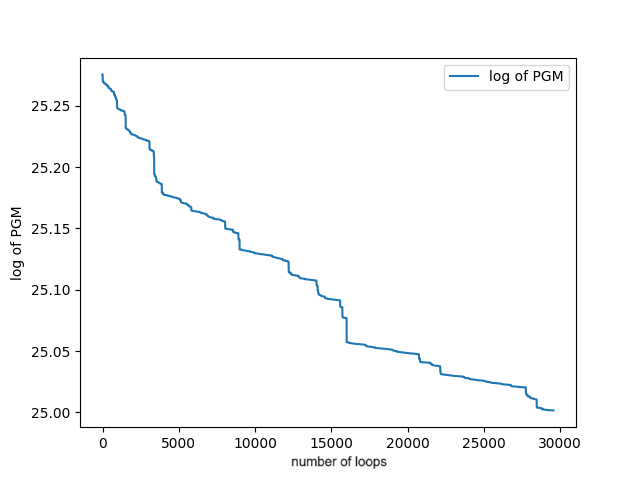
\includegraphics[width=100mm]{100.png}
    \caption{$100$次元における$\log \mathrm{PGM}$の挙動}
\end{figure}

%![$80$次元における$\log \mathrm{PGM}$の挙動](/uploads/mathdown/Ma4HAumZMz6UXvBSgtUG.png)

%![$100$次元における$\log \mathrm{PGM}$の挙動](/uploads/mathdown/p06C2unHxn3Ho9VGGsfu.png)

\subsection{RHFの比較}
まず,格子基底のRHFとは次のように定義されるものです.

\begin{definition}[Root of Hermite factor(RHF)]
    格子基底$\{\boldsymbol{b}_1,\ldots,\boldsymbol{b}_n\}$の\textbf{root of Hermite factor}もしくは\textbf{RHF}とは
    
    $$
    \mathrm{rhf}(\boldsymbol{b}_1,\ldots,\boldsymbol{b}_n)\coloneqq \sqrt[n]{\frac{\norm{\boldsymbol{b}_1}}{\sqrt[n]{\mathrm{vol}(\boldsymbol{b}_1,\ldots,\boldsymbol{b}_n)}}}
    $$
    
    である.
\end{definition}

SVP Challengeのseed0,$40$次元~$150$次元までの基底に関して簡約パラメタ$\delta=0.99$でのLLL,PGMLLL,そしてブロックサイズ$\beta=10, 15$でのBKZを施し,RHFをプロットしました.ただし,LLLは$\texttt{SageMath}$の$\texttt{LLL}$関数をBKZは$\texttt{NTL}$ライブラリの$\texttt{BKZ\_FP}$関数を利用しました.

\begin{figure}[H]
    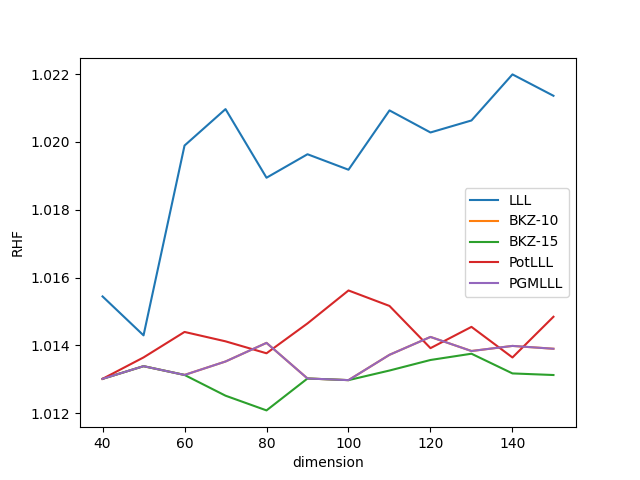
\includegraphics[width=100mm]{RHF40-150.png}
    \caption{RHFの比較}
\end{figure}

%![RHFの比較](/uploads/mathdown/90Ls8G3IL857T0z2sWTh.png)

図4から,少なくとも150次元程度まででは,ブロックサイズ$\beta=10$のBKZと同じ品質であり,ブロックサイズ$\beta=15$のBKZとほぼ同程度の品質を維持することがわかります.

\end{document}
